% ===== 04_sensitivity =====
\section{成本与参数敏感性}
\label{sec:cost}
前一节确定了给定参数下的控制过程。阈值改变时，启动状态和控制持续时间同时改变；传播及常规控制参数还会改变退出状态。因此，对控制指标求导时不能把 $S^*$ 或 $S_c$ 当作固定的外部输入。本节先分析启动状态，再讨论感染阈值与常规接触率的影响。

除特别说明外，以下偏导数均固定 $N,S_0,I_0$ 及其余独立参数，并在相应触发条件的内部讨论。$\eta$ 作为独立设计参数；若它随其他参数同步调整，相应总变化应按复合函数求导。在 $q_0=0$ 或 $\beta=1$ 的边界，涉及该参数的导数理解为允许参数侧的单侧导数。$S_c,S_q,q_c$ 中的下标均按变量定义使用，不表示求导。

\subsection{干预成本与启动状态的参数导数}
为比较两种干预，保留线性强度积分
\begin{equation}
J_c=\int_{t_1}^{t_2}\frac{(c_0-c(t))_+}{c_0}\,dt,
\qquad
J_q=\int_{t_1}^{t_2}\frac{(q(t)-q_0)_+}{1-q_0}\,dt,
\label{eq:cost:linear}
\end{equation}
并采用二次加权成本
\begin{equation}
J=\int_{t_1}^{t_2}\left[
\left(\frac{(c_0-c(t))_+}{c_0}\right)^2
+2\left(\frac{(q(t)-q_0)_+}{1-q_0}\right)^2\right]dt,
\label{eq:cost:J}
\end{equation}
其中 $(x)_+=\max\{x,0\}$。$J$ 不等于 $J_c+2J_q$。该指标累计相对于常规水平的归一化干预强度；当时间以天计时，$J$ 的单位为天，而不是货币。它也不直接计入隔离人数或隔离期间的资源占用。仅隔离控制有 $J_c=0$；联合控制仍使用同一个 $J$，以保持比较口径一致。

\begin{lemma}
\label{lem:s1:Sstar-sensitivity}
在条件\eqref{eq:model:trigger}下，启动状态满足
\begin{equation}
\frac{\partial S^*}{\partial\eta}<0,\qquad
\frac{\partial S^*}{\partial c_0}>0,\qquad
\frac{\partial S^*}{\partial\beta}>0,\qquad
\frac{\partial S^*}{\partial q_0}<0.
\label{eq:s1:Sstar-signs}
\end{equation}
\end{lemma}
\begin{proof}
令
\[
F(S;\eta,c_0,\beta,q_0)
=I_0+\frac{\beta_2^0}{\beta_1^0}(S_0-S)+\rho_1\ln(S/S_0)-\eta.
\]
在 $S=S^*>S_c$ 处，
\[
\frac{\partial F}{\partial S}=\rho_1\left(\frac1{S^*}-\frac1{S_c}\right)<0.
\]
因此隐函数定理适用。$\partial F/\partial\eta=-1$，而在固定 $S=S^*$ 时
\begin{align*}
\frac{\partial F}{\partial c_0}
&=-\frac{\rho_1}{c_0}\ln\frac{S^*}{S_0}>0,\\
\frac{\partial F}{\partial\beta}
&=\frac{q_0(1-q_0)}{[\beta+q_0(1-\beta)]^2}(S_0-S^*)
-\frac{\rho_1(1-q_0)}{\beta+q_0(1-\beta)}\ln\frac{S^*}{S_0}>0,\\
\frac{\partial F}{\partial q_0}
&=-\frac{\beta}{[\beta+q_0(1-\beta)]^2}\left[(S_0-S^*)-\bar S\ln\frac{S_0}{S^*}\right]<0.
\end{align*}
最后一个符号使用 $\bar S<S^*<S_0$ 及 $\ln x<x-1$。由
$\partial S^*/\partial p=-(\partial F/\partial p)/(\partial F/\partial S)$ 即得所列符号。特别地，
\begin{equation}
\frac{\partial S^*}{\partial\eta}
=\frac1{\rho_1(1/S^*-1/S_c)},\qquad
\frac{\partial S^*}{\partial c_0}
=\frac{\ln(S^*/S_0)}{c_0(1/S^*-1/S_c)}.
\label{eq:s1:Sstar-eta-sign}
\end{equation}
另两个偏导数的完整表达为
\begin{align}
\frac{\partial S^*}{\partial\beta}
&=\frac{\dfrac{q_0(1-q_0)(S_0-S^*)}{[\beta+q_0(1-\beta)]^2}
-\dfrac{\rho_1(1-q_0)}{\beta+q_0(1-\beta)}\ln(S^*/S_0)}
{\rho_1(1/S_c-1/S^*)},\label{eq:s1:Sstar-beta-sign}\\
\frac{\partial S^*}{\partial q_0}
&=-\frac{\beta[(S_0-S^*)-\bar S\ln(S_0/S^*)]}
{[\beta+q_0(1-\beta)]^2\rho_1(1/S_c-1/S^*)}.
\label{eq:s1:Sstar-q0-sign}
\end{align}
固定 $N$ 且使用 $\theta=\eta/N$ 时，有 $\partial S^*/\partial\theta=N\partial S^*/\partial\eta$。
\end{proof}

\subsection{感染阈值与控制负担的权衡}
提高阈值推迟启动，使控制开始时的易感者人数减小。这一变化同时影响所需最大隔离比例、持续时间和累计感染，而这些指标的方向并不相同。
\begin{proposition}
\label{prop:threshold-tradeoff}\label{prop:s1:sensitivity}
对于仅隔离控制，在触发区间内有
\begin{equation}
\frac{\partial t_1}{\partial\eta}>0,\quad
\frac{\partial q_{\max}}{\partial\eta}<0,\quad
\frac{\partial\Delta t}{\partial\eta}<0,\quad
\frac{\partial J_q}{\partial\eta}<0,\quad
\frac{\partial J}{\partial\eta}<0.
\label{eq:threshold-tradeoff}
\end{equation}
若进一步有 $\eta>1$，则 $\partial\Itcum/\partial\eta>0$。计算至无限时刻的累计新增感染也随 $\eta$ 严格增加。
\end{proposition}
\begin{proof}
由式\eqref{eq:s1:t1}及 $I(S^*)=\eta$，
\[
\frac{\partial t_1}{\partial\eta}
=-\frac1{\beta_1^0 S^*\eta}\frac{\partial S^*}{\partial\eta}>0.
\]
式\eqref{eq:s1:qmax}给出
$\partial q_{\max}/\partial\eta=\gamma N[\beta c_0(S^*)^2]^{-1}\partial S^*/\partial\eta<0$。
控制时长满足
\[
\frac{\partial\Delta t}{\partial\eta}
=-\frac{\Delta t}{\eta}
+\frac{N}{c_0\eta(S^*-\bar S)}\frac{\partial S^*}{\partial\eta}<0.
\]
又由于 $(q_c(S)-q_0)/(1-q_0)=1-S_c/S$，有
\begin{equation}
J_q=\frac{N}{c_0\eta}\int_{S_c}^{S^*}\frac{1-S_c/S}{S-\bar S}\,dS,
\qquad
J=\frac{2N}{c_0\eta}\int_{S_c}^{S^*}\frac{(1-S_c/S)^2}{S-\bar S}\,dS.
\label{eq:cost:state}
\end{equation}
被积函数不含 $\eta$ 且在区间内部为正，系数 $1/\eta$ 和上限 $S^*$ 均随 $\eta$ 减小，故两个成本严格下降。两积分的初等表达列于附录\ref{app:cost}。

为分析累计感染，退出后 $I=1$ 的条件对 $\eta$ 求导得
\[
\frac{\partial S_{\rm end}}{\partial\eta}
=-\frac1{\rho_1(1/S_{\rm end}-1/S_c)}<0.
\]
对式\eqref{eq:s1:cumulative}求导，
\begin{equation}
\frac{\partial\Itcum}{\partial\eta}
=\left[\frac{\beta S^*}{S^*-\bar S}-\frac{\beta}{\beta+q_0(1-\beta)}\right]\frac{\partial S^*}{\partial\eta}
-\frac{\beta}{\beta+q_0(1-\beta)}\frac{\partial S_{\rm end}}{\partial\eta}>0.
\label{eq:cumulative-eta}
\end{equation}
其中使用 $\beta S_c/(S_c-\bar S)=\beta/[\beta+q_0(1-\beta)]$，以及 $S/(S-\bar S)$ 在 $S>\bar S$ 上非增。因此方括号非正，其与 $\partial S^*/\partial\eta<0$ 的乘积非负，最后一项严格为正。将终点替换为 $I=0,S=S_\infty$，同样的隐式微分给出无限时刻的结论。
\end{proof}
该命题给出阈值选择的一项基本限制：允许更高的社区感染水平会降低额外干预强度及其持续时间，却增加累计感染。这里没有据此断言动态清零时间对任意参数都具有相同单调性；它还包括退出后的下降过程。

\subsection{常规接触率与控制持续时间}
改变 $c_0$ 不仅改变传播速度，也改变 $S_c$。因此，先需要确定哪些接触率会触发控制。固定其余参数，当
\[
c_0\le\frac{\gamma N}{\beta(1-q_0)S_0}
\]
时，常规峰值为 $I_0$；超过该值后，式\eqref{eq:s1:Imax-no}给出
\begin{equation}
\frac{dI_{\max}^{no}}{dc_0}
=-\frac{\rho_1}{c_0}\ln\frac{S_c}{S_0}>0.
\label{eq:s1:Imax-no-c0-derivative}
\end{equation}
此时峰值从 $I_0$ 严格增加至 $I_0+\beta_2^0 S_0/\beta_1^0$。若
\[
I_0<\eta<I_0+\frac{\beta_2^0}{\beta_1^0}S_0,
\]
则唯一的临界常规接触率 $c_{0,\min}(\eta)$ 满足
\begin{equation}
I_{\max}^{no}\bigl(c_{0,\min}(\eta)\bigr)=\eta,
\qquad c_{0,\min}(\eta)>\frac{\gamma N}{\beta(1-q_0)S_0}.
\label{eq:s1:c0-min-def}
\end{equation}
正持续时间的控制恰在 $c_0>c_{0,\min}(\eta)$ 时触发。

\begin{proposition}
\label{prop:contact-effects}\label{cor:s1:duration-sensitivity}
在触发条件内部，对于仅隔离控制，
\[
\frac{\partial t_1}{\partial c_0}<0,\qquad
\frac{\partial q_{\max}}{\partial c_0}>0,\qquad
\frac{\partial\Delta t}{\partial\beta}>0,\qquad
\frac{\partial\Delta t}{\partial q_0}<0.
\]
接触率对控制持续时间的影响由
\begin{equation}
\frac{\partial\Delta t}{\partial c_0}
=\frac{N}{c_0^2\eta}
\left\{\frac{S^*}{S^*-\bar S}
\left[1+\frac{S_c}{S^*-S_c}\ln\frac{S_0}{S^*}\right]
-\ln\frac{S^*-\bar S}{S_c-\bar S}\right\}
\label{eq:duration-c0}
\end{equation}
确定，其符号不能统一为正或负。固定 $I_0<\eta<I_0+\beta_2^0S_0/\beta_1^0$ 时，$\Delta t$ 在 $c_0\in(c_{0,\min},\infty)$ 内至少有一个极大值，但不据此断言极大值唯一。
\end{proposition}
\begin{proof}
写 $I(S;c_0)=I_0+\frac{\beta_2^0}{\beta_1^0}(S_0-S)+\rho_1\ln(S/S_0)$。在 $S<S_0$ 时，
\[
\frac{\partial I(S;c_0)}{\partial c_0}=-\frac{\rho_1}{c_0}\ln\frac{S}{S_0}>0.
\]
式\eqref{eq:s1:t1}中的前置系数 $1/\beta_1^0$ 随 $c_0$ 下降，下限 $S^*$ 随 $c_0$ 上升，被积函数也下降；逐项求导均给出负项，故 $\partial t_1/\partial c_0<0$。同时
\[
\frac{\partial q_{\max}}{\partial c_0}
=\frac{\gamma N}{\beta c_0^2(S^*)^2}
\left(S^*+c_0\frac{\partial S^*}{\partial c_0}\right)>0.
\]
对 $\Delta t$ 的对数因子求导时，
\[
\frac{\partial\bar S}{\partial\beta}=-\frac{\gamma N}{c_0\beta^2}<0,
\qquad
\frac{\partial(S_c-\bar S)}{\partial\beta}=-\frac{q_0S_c}{\beta}\le0.
\]
结合 $\partial S^*/\partial\beta>0$ 得 $\partial\Delta t/\partial\beta>0$。
由于 $\bar S$ 不含 $q_0$，而 $\partial S^*/\partial q_0<0$、$\partial S_c/\partial q_0=S_c/(1-q_0)>0$，得到 $\partial\Delta t/\partial q_0<0$。
利用 $\partial\bar S/\partial c_0=-\bar S/c_0$、$\partial S_c/\partial c_0=-S_c/c_0$ 及式\eqref{eq:s1:Sstar-eta-sign}，直接整理得到式\eqref{eq:duration-c0}。

当 $c_0\downarrow c_{0,\min}$ 时，$S^*\to S_c$，所以 $\Delta t\to0$。当 $c_0\to\infty$ 时，启动方程给出
$S^*\to S_0-\frac{\beta_1^0}{\beta_2^0}(\eta-I_0)>0$，而 $S_c,\bar S$ 均为 $O(c_0^{-1})$，故
\[
\Delta t=\frac{N}{c_0\eta}[\ln c_0+O(1)]\longrightarrow0.
\]
$\Delta t$ 在内部为正且连续，两端趋零，因此在内部达到正的最大值；中值定理同时保证其导数取正、负两种符号。
\end{proof}
式\eqref{eq:duration-c0}也给出原有的等价符号判据：
\begin{equation}
\frac{\partial\Delta t}{\partial c_0}\gtrless0
\quad\Longleftrightarrow\quad
\ln\frac{S_0}{S^*}\gtrless
\frac{S^*-S_c}{S_c}
\left[\frac{S^*-\bar S}{S^*}\ln\frac{S^*-\bar S}{S_c-\bar S}-1\right],
\label{eq:duration-c0-equivalent}
\end{equation}
等号亦相应成立。特别地，若右端不大于零，则导数严格为正。这一判据由式\eqref{eq:duration-c0}乘以正因子后整理得到，无需再为右端引入符号。

与阈值 $\eta$ 的影响不同，较高接触率使干预更早启动且要求更大的隔离比例，却未必对应更长的控制时间。这一差别来自起止状态和时间尺度共同变化，而非控制强度与持续时间之间的直接对应。

\subsection{人口归一化与低阈值极限}
\label{sec:scaling-theory}
记 $s=S/N,i=I/N,\theta=\eta/N$。固定归一化初值时，人数尺度可从二维方程中消去；这与固定绝对初始感染人数是不同的比较方式。固定阈值比例与固定绝对阈值是两种不同的设计情景。
\begin{proposition}
\label{prop:scaling}
对于仅隔离控制，固定 $s_0,i_0$ 和 $\beta,\gamma,c_0,q_0$。在阈值控制被触发时，$t_1,\Delta t,q_{\max},J$ 以及存在内部拐点时的 $\lambda$ 对 $N,\eta$ 的依赖仅通过 $\theta=\eta/N$ 表现。最终累计新增感染除以 $N$ 后亦不依赖 $N$。但是，使用绝对终点 $I=1$ 时，$t_{\rm end}$ 及计算至该终点的累计感染比例一般仍含 $N$。
\end{proposition}
\begin{proof}
常规阶段的归一化系统为
\[
\dot s=-c_0[\beta+q_0(1-\beta)]si,\qquad
\dot i=[\beta c_0(1-q_0)s-\gamma]i.
\]
它不含 $N$，触发条件为 $i=\theta$，所以 $t_1$ 与 $s^*=S^*/N$ 仅依赖上述固定量和 $\theta$。又
\[
s_c=\frac{\gamma}{\beta c_0(1-q_0)},\qquad
\bar s=\frac{(1-\beta)\gamma}{\beta c_0},\qquad
\Delta t=\frac1{c_0\theta}\ln\frac{s^*-\bar s}{s_c-\bar s}.
\]
例如，二次成本的归一化表达为
\begin{equation}
J=\frac{2}{c_0\theta}\int_{s_c}^{s^*}
\frac{(1-s_c/s)^2}{s-\bar s}\,ds,
\label{eq:dom:Jtheta}
\end{equation}
其中仅含归一化状态和固定参数。代入控制表达可得其余结论。无限时间的终点为 $i\to0$，同样不含 $N$；有限的操作性终点却为 $i=1/N$，因而保留绝对人口尺度。
\end{proof}

若固定 $i_0>0$，允许的阈值为 $\theta>i_0$，不能直接在这一固定初值问题中令 $\theta\to0$。沿同时满足 $i_0\to0$、$\theta\to0$、$0<i_0<\theta$ 的序列，且 $s_0$ 趋于某个大于 $s_c$ 的固定值时，有 $s^*\to s_0$，从而
\begin{equation}
\Delta t\sim\frac1{c_0\theta}\ln\frac{s_0-\bar s}{s_c-\bar s},\qquad
J\sim\frac2{c_0\theta}\int_{s_c}^{s_0}\frac{(1-s_c/s)^2}{s-\bar s}\,ds.
\label{eq:small-threshold}
\end{equation}
两者均按 $1/\theta$ 的量级发散。相反，在固定 $i_0>0$ 时令 $\theta\downarrow i_0$，控制持续时间趋于有限值
\[
\frac1{c_0i_0}\ln\frac{s_0-\bar s}{s_c-\bar s}.
\]
因此，基于时长或成本反函数定义的阈值边界应限定在相应值域内；不能将联合小初值极限用于固定正初值的反函数结论。


% ===== 04_numerical_illustrations =====
\subsection{参数敏感性的数值图示}
参数取值见各图图注。图\ref{fig:baseline:q-joint}给出不同 $c_0$ 与 $\eta$ 下的隔离率轨迹。图\ref{fig:scenario1_heatmaps_c0_eta}则展示相关指标在同一参数平面内的变化；触发边界下方无需加强隔离。代表数值见第\ref{sec:numerics}节及补充表\ref*{tab:sup:baseline}。

\begin{figure}[htbp]
\centering
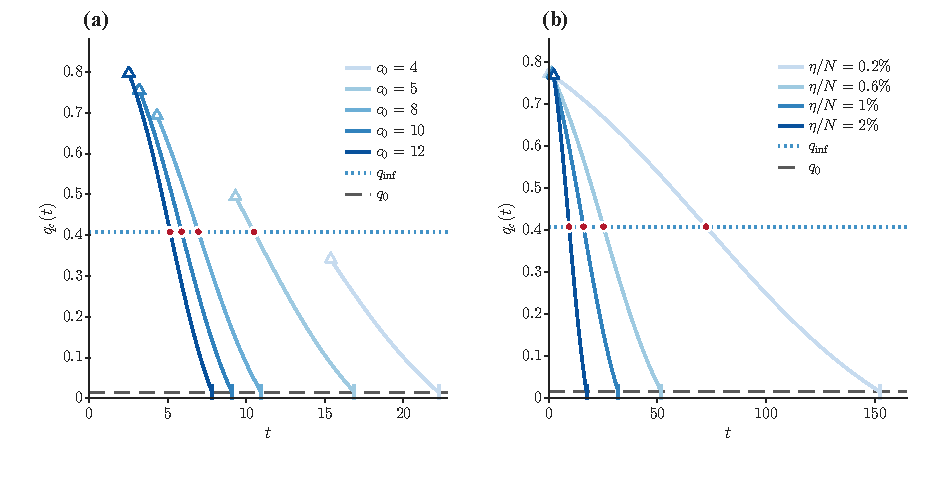
\includegraphics[width=\textwidth]{figures/layout_v5/baseline_q_joint.pdf}
\caption{不同常规接触率和感染阈值下的隔离率轨迹。固定 $N=763,S_0=762,I_0=1,\beta=0.155,\gamma=0.3504\ \mathrm d^{-1},q_0=0.01526$。(a) 固定 $\eta/N=5\%$，$c_0=4,5,8,10,12$；(b) 固定 $c_0=10$，$\eta/N=0.2\%,0.6\%,1\%,2\%$。三角形、短竖线分别表示 $t_1,t_2$，红点为内部拐点。水平虚线为 $q_0$，点线为 $\qinf$。$c_0=4$ 时不存在内部拐点。横轴 $t$ 的单位为天。}
\label{fig:baseline:q-joint}
\end{figure}

\begin{figure}[htbp]
\centering
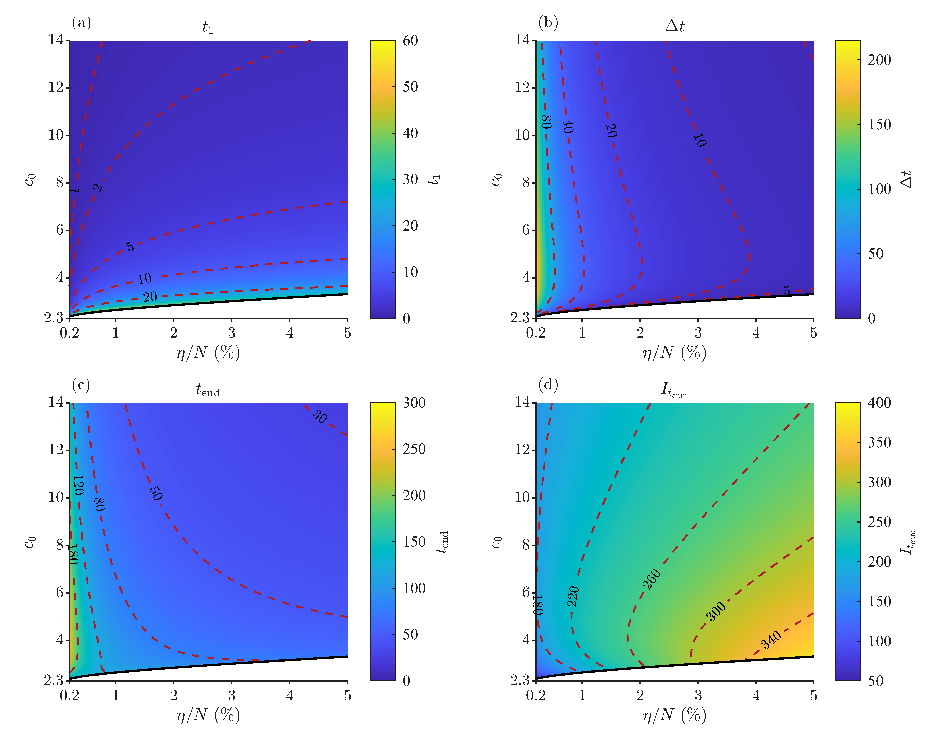
\includegraphics[width=0.8\textwidth]{figures/scenario1_heatmaps_c0_eta.pdf}
\caption{$(\eta/N,c_0)$ 平面上的启动时间、控制持续时间、清零时间和累计感染。固定 $N=763,S_0=762,I_0=1,\beta=0.155,\gamma=0.3504\ \mathrm d^{-1},q_0=0.01526$。实线为触发边界 $c_{0,\min}(\eta)$，白色区域无需加强隔离，虚线为各指标的等值线。}
\label{fig:scenario1_heatmaps_c0_eta}
\end{figure}


\FloatBarrier

